\documentclass[
    11pt,
    spanish,
	a4paper
]{article}
\usepackage[utf8]{inputenc}
\usepackage[spanish]{babel}
\usepackage{graphicx}
\usepackage{authoraftertitle}
\usepackage{float}
\usepackage{caption}
\usepackage{verbatim}
\usepackage{listings}
\captionsetup[table]{labelformat=empty}

\def\doctype{Trabajo práctico}
\title{EDU-CIAA}
\author{Gonzalo Nahuel Vaca}

\begin{document}

\makeatletter
\begin{titlepage}
	\begin{center}
		\vspace*{1cm}
		
		\Huge
		\textbf{\doctype}
		\vspace{0.5cm}
    
		\LARGE
		\@title
		\vspace{0.5cm}
    
		\textbf{Procesamiento Digital de Señales (fundamentos)}
		
		\vspace{1.5cm}
		
		\textbf{\@author}

		\vspace{1.5cm}

		
\includegraphics[width=0.8\textwidth]{img/logoFIUBA.pdf}
		
		\vfill
		Maestría en Sistemas Embebidos\\
		Universidad de Buenos Aires\\
		Argentina\\
		\today
	\end{center}
\end{titlepage}
\makeatother
\newpage

\section{Resolución punto 1}

Dado dos números de N bits, su producto necesariamente consumen 2N bits.
Al expresar el resultado como N bits se trunca el valor.
En este caso, el valor real es 0x1180 sin embargo se truncó hasta dejar 0x11
para que pueda entrar en q7.
Esto deforma el valor.

En la figura \ref{fig:term1} se puede observar la captura de los datos calculados.

\begin{figure}[htbp]
	\centering
	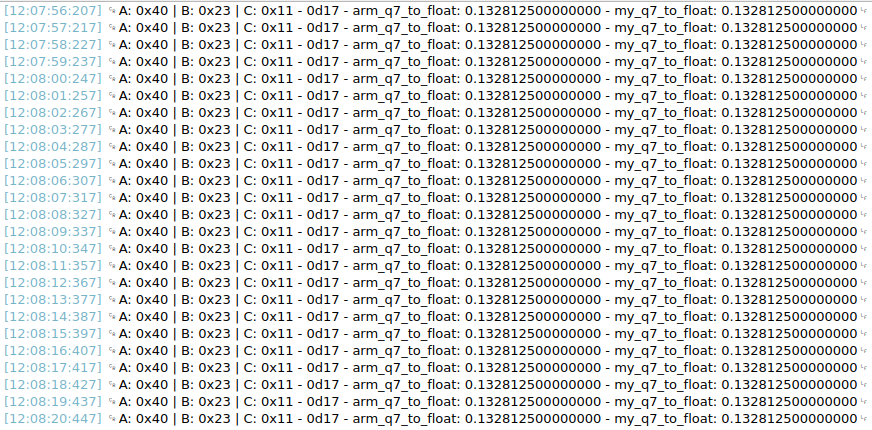
\includegraphics[width=\textwidth]{img/cutecom01.png}
	\caption{Captura de terminal serie del ejercicio 1.}
	\label{fig:term1}
\end{figure}


\end{document}